\documentclass[a4paper,oneside]{memoir}
\usepackage[english]{babel}
\usepackage[T1]{fontenc}
\usepackage[utf8]{inputenc}
\usepackage{wallpaper}
\usepackage{palatino}
\usepackage{hyperref}
\usepackage{csquotes}
\usepackage{listings}
\usepackage{float}
\usepackage{wrapfig}
\restylefloat{figure}
%linespacing
\usepackage{setspace}
\renewcommand{\baselinestretch}{1.5}

% Bibliography
\usepackage[style=authoryear]{biblatex}
\addbibresource{bib.bib}
\bibliography{bib}

% Promote sections and subsections
\setheadfoot{\onelineskip}{2\onelineskip}
\setheaderspaces{*}{1mm}{*}
% \chapterstyle{plain} % needed?
\checkandfixthelayout

% \renewcommand{\thesection}{\arabic{section}}
% \makeatletter
% \let\l@section\l@chapter
% \makeatother
% %
% % \renewcommand{\thesection}{\arabic{section}}
% % \renewcommand{\thesubsection}{\thesection.\arabic{subsection}}
% % \makeatletter
% % \let\l@subsection\l@section
% % \let\l@section\l@chapter
% % \makeatother

% Glossary
\usepackage[numberedsection=nameref]{glossaries}
\renewcommand{\glossarypreamble}{\label{glos}}
\makeglossaries
\newglossaryentry{ai} {
    name = artificial intelligence,
    description = {Artificial intelligence (AI) covers the broad discipline in computer science
that is concerned with replicating intelligent behaviour in computational systems. The exact
definition is controversial for historical reasons \autocite{Nilsson2009}}
}
\newglossaryentry{computation} {
   name = computation,
   description = {Computation refers to any process (in any
substrate) that can deduce new information based on old information. In
this is manifested as computing instructions}
}
\newglossaryentry{dsl} {
  name = domain specific language,
  description = {A DSL is a language used to model concepts from a certain
    domain. DSLs are usually simpler than more general programming languages in
    that they contain fewer concepts and less complex syntax}
}
\newglossaryentry{futhark} {
   name = {Futhark},
   description = {A programming language geared towards performance in parallel environment such as
   graphics processors (GPUs). Futhark is a purely functional array language and is
   developed by HIPERFIT research center under the Department of Computer Science at the
   University of Copenhagen (DIKU)}
}
\newglossaryentry{ncc} {
   name = {NCC},
   description = {Neural patterns or condition that is minimally sufficient for a conscious
thought to occur. See \autocite{atkinson2000, Hohwy2009}}
}
\newglossaryentry{ml} {
  name = machine learning,
  description = {Machine learning is a sub-field within \gls{ai} that is concerned
    with developing systems that "progressively improves their performance on a
    certain task" \autocite{wiki:ml}}
}
\newglossaryentry{meme} {
name = meme,
description = {\textit{Meme} is a shortened form of the ancient Greek \textit{mimeme} meaning
'imitated thing' and was coined by Richard Dawkins. A meme refers to a idea or a
\textit{way of behaving} that can be \enquote{copied, transmitted, remembered, taught, shunned,
brandished, ridiculed, parodied, censored, hallowed} \autocite{dennett2017}}
}
\newglossaryentry{opencl} {
   name = {OpenCL},
   description = {An open standard for cross-platform parallel programming, which
   allows software to be executed on CPUs, GPUs or other processors or hardware accelerators. See \url{
   https://www.khronos.org/opencl/}}
}
\newglossaryentry{ref} {
  name = REF,
  description = {A model for rehabilitation in patients with brain lesions, developed
    by \cite{Mogensen2011}. An extension in the form of the REFGEN model was developed by
    \cite{Mogensen2017}}
}

\makeglossaries
% Setup captions
\captionstyle[\centering]{\centering}
\changecaptionwidth
\captionwidth{0.8\linewidth}

% Protect against widows and orphans
%\clubpenalty=10000
%\widowpenalty=10000

%\linespread{1.2}

\raggedbottom

\chapterstyle{ger}

\maxsecnumdepth{subsection}

% Change memoir chapter margins
\usepackage{titlesec}
\titleformat{\chapter}[display]
{\normalfont\huge\bfseries}{\chaptertitlename\ \thechapter}{5pt}{\Huge}
\titlespacing*{\chapter}{10pt}{10pt}{10pt}

%%  Setup fancy style quotation
%%  ==================================================================
%\usepackage{tikz}
%\usepackage{framed}

%\newcommand*\quotefont{\fontfamily{fxl}} % selects Libertine for quote font

% Make commands for the quotes
%\newcommand*{\openquote}{\tikz[remember picture,overlay,xshift=-15pt,yshift=-10pt]
%     \node (OQ) {\quotefont\fontsize{60}{60}\selectfont``};\kern0pt}
%\newcommand*{\closequote}{\tikz[remember picture,overlay,xshift=15pt,yshift=5pt]
%     \node (CQ) {\quotefont\fontsize{60}{60}\selectfont''};}

% select a colour for the shading
%\definecolor{shadecolor}{rgb}{1,1,1}

% wrap everything in its own environment
%\newenvironment{shadequote}%
%{\begin{snugshade}\begin{quote}\openquote}
%{\hfill\closequote\end{quote}\end{snugshade}}

%%  Begin document
%%  ==================================================================
\begin{document}

%%  Begin title page
%%  ==================================================================
    \thispagestyle{empty}
    \ULCornerWallPaper{1}{ku-coverpage/nat-farve.pdf}
    \ULCornerWallPaper{1}{ku-coverpage/diku-en.pdf}
    \begin{adjustwidth}{-3cm}{-1.5cm}
    %\vspace*{-1cm}
    %\textbf{\Huge Free topic} \\
    \vspace*{2.5cm}
    \textbf{\Huge Modelling learning systems} \\
    \vspace*{.8cm}
    {\huge  A DSL for cognitive neuroscientists}\\
    \begin{tabbing}
    % adjust the hspace below for the longest author name
    Jens Egholm Pedersen \hspace{1cm} \= \texttt{<xtp778@alumni.ku.dk>} \\
    \\[11cm]

    \textbf{\Large Supervisor} \\
    Martin Elsman \hspace{1cm} \texttt{<mael@di.ku.dk>}
    \end{tabbing}
    \end{adjustwidth}

    \newpage

    \ClearWallPaper
%%  ==================================================================
%%  End title page

\renewcommand\cftchapteraftersnumb{\normalfont}
\renewcommand\cftbeforechapterskip{5pt plus 1pt}

\vspace*{\fill}
\begin{center}
\textbf{Acknowledgements}
\end{center}
\begin{center}
\begin{minipage}{.8\textwidth}

I would like to thank the Unit for Cognitive Neuroscience in Copenhagen for
the many talks and assistance in the making of this paper. The patience of
Nicolaj Daugaard and Jesper Mogensen in particular deserves high praise.
\end{minipage}
\end{center}
\vfill

\newpage

\frontmatter
\tableofcontents*
\newpage

\mainmatter
\chapter{Introduction}
In the past years machine learning has surpassed humans in some recognition
tasks, and the development shows no signs of slowing down.
These developments are however based on relatively old research on neural
networks \autocite{Nilsson2009, russel2007}.
Newer investigation into rehabilitation and learning indicates that such
networks alone cannot account for the same amount of learning that happens
in the brain \autocite{Mogensen2011, block2007, russel2007, Moravec98, dennett2017}.
For that reason the breakthroughs in machine learning are hard to transfer
to the domain of cognitive neuroscience.

As an attempt to remedy this, this project sets out to define a domain-specific
language (DSL) that is capable of representing learning systems that resemble
those from the domain of neuroscience.

The second part of the paper validates this DSL through the modelling of a small
learning task. The benchmark will be written in \gls{futhark} and compiled to
the \gls{opencl} standard. The language abstraction however, allows it to be
executed on any machine architecture.

The goal is for the DSL to explore a more accurate scientific representation of
learning and learning concepts, serving as a more approachable simulation tool
for the cognitive neurosciences.

\section{Problem statement}
Building on theories and concepts of the domain of cognitive neuroscience
this paper examines the hypothesis that
\textit{
  the DSL presented in this paper can model meaningful machine learning
  tasks for the cognitive neurosciences,
  agnostic of the learning system implementation}.
The paper will approach this in two steps:

\begin{enumerate}
  \item Defining and implementing a DSL abstraction for the expression of
        learning tasks, based on the REF model from \autocite{Mogensen2011}.
  \item Testing the DSL by expressing a learning task in a Krechevsky
        T-maze \autocite{Krechevsky1932}, backed by a traditional machine
        learning implementation in \gls{futhark}.
\end{enumerate}
%
% \section{Structure}
% This paper is built around theoretical concepts from cognitive neuroscience,
% \gls{ml} and finally

{\let\clearpage\relax\chapter{Theoretical Foundations}}
This section accounts for the theoretical foundation of the paper and is divided
into three parts.
The first part concerns the broad topic of computation and learning in neural
systems as seen from the perspective of computational neuroscience. By focusing
on cognition, plasticity, learning and rehabilitation, it derives
the necessary and sufficient language abstractions to capture the complexity
of the domain.
The second part introduces traditional machine learning from the perspective of
computer science. These concepts will be applied in the validation phase of
learning model abstractions in section \ref{case}.
In the final part the theoretical and methodological background for the
development of \gls{dsl}s will be treated.

\section{Learning in neural systems}
\begin{quote}
  Activity-dependent synaptic plasticity is widely believed to be the basic
  phenomenon underlying learning and memory \autocite{dayan2001}.
\end{quote}

Commonly referred to as \textit{what fires together, wires together}, Hebbian
learning suggests that synaptic connections from neuron $A$ to neuron $B$
are strengthened or weakened when neuron $A$ excites or inhibits the chance of
firing neuron $B$ respectively \autocite{dayan2001}.
Hebbian learning is believed to play a large part in the plastic nature of the
brain, especially within learning and memory formation
\autocite{dayan2001, Johnston2009, Robertson1999}.

\subsection{Reorganisation of elementary functions}
\label{ref}

\autocite{Robertson1999} studied patients during
rehabilitation of brain damage and conjectured that learning --- either when
acquiring new information or recovering from lost information --- occurs based
on the structural changes induced by the Hebbian principle
\autocite{Robertson1999}. They further concluded that the damaged brain areas
regenerate themselves based on this principle \autocite{Robertson1999}.
Mogensen refutes this point by claiming that, while there
may be some synaptogenesis, the rehabilitation mainly occurs when other parts
of the brain learns to take over the lost functions \autocite{Mogensen2011}.

Mogensen arrives at a theoretical framework which divides the
brain into localized and highly specialised, basic information
processing elementary functions (EF). These modular functions are contained
in a \textit{substructure} or \textit{local circuit}
within the brain \autocite{Mogensen2011}.

Multiple EFs interact to form algorithmic strategies (AS), established as
a consequence of learning and experiencing \autocite{Mogensen2011}. An
algorithmic strategy combines the capacity of multiple EFs into a single - and
for the AS appropriate - response \autocite{Mogensen2011, Mogensen2012b}.

The EF and AS interplay to create what Mogensen dubbed '\textit{surface
phenomena}', which manifests the behaviour of the system \autocite{Mogensen2011}.
Surface phenomena are the product of applying an AS to a particular problem,
and Mogensen hypothesised that a given AS is evaluated for every success or
failure of the surface behaviour predicted by that AS \autocite{Mogensen2011}.
Such evaluation either strengthens the AS's association with the given
behaviour scenario, or weakens it, potentially starting a search for another
AS to perform the task instead \autocite{Mogensen2011}.
According to Mogensen these changes are controlled by a specialised AS dubbed
the \textit{Supervisory Attentional System} (SAS) from \autocite{Norman1986},
manifested through neuroplastic changes in the synaptic connections within
the SAS \autocite{Mogensen2011}.

\textit{Behaviour} in the \gls{ref} model is thus defined as the response of a single
AS to a given task, that in turn consists of a number of EFs
\autocite{Mogensen2011, Mogensen2012b}.

%In an addition to the REF model, Mogensen introduced the algorithmic
%module (AM), which is a module similar to an AS, but whose computations can be
%shared by many AS \autocite{Mogensen2012b}. In other words they may not
%directly mediate "a task solution", but partake in many different task
%situations \autocite{Mogensen2017}.

An elaboration to the \gls{ref} model arrived in the form of the REFGEN
model (general reorganisation of elementary functions) \autocite{Mogensen2017}.
The REFGEN model further explains the feedback mechanisms of the SAS
to account for the 'learning' or adaptive feature of neural systems, by
introducing two new concepts: the goal algorithmic strategy (GAS) and the
comparator \autocite{Mogensen2017, Mogensen2012b}.

In this new framework the SAS is tasked with maintaining the current state
of the system, while the GAS reflects the goal towards which it is desired to
to move, for instance the exit condition in a maze \autocite{Mogensen2017}.
For this to be useful a comparator is needed to constantly compare the SAS
and GAS (the current state versus the goal), such as to select the optimal AS
for the task at hand \autocite{Mogensen2017}. The feedback (backpropagation)
from the actuation on the surrounding world is received by the comparator,
who will assert influence on the SAS and GAS to better account for the new
reality \autocite{Mogensen2017}.

% TODO: Write about the reality -> encoding -> brain -> decoding -> reality loop

\section{Learning in machines}
Systems that display the capability of learning (or progressively improving on
a certain task) are historically associated with the field of \gls{ml}.
\Gls{ml} goes back to the 1950s, and is tightly coupled
with artificial intelligence --- the idea of creating intelligence
in machines \autocite{Nilsson2009, russel2007}.
It is a large and active research field, and this is why this section will strictly
focus on a brief introduction and motivation of the topic in the context of
learning tasks. This will be followed by a more in-depth description of
multilayered perceptron networks and progressive learning through stochastic
gradient descent. Both techniques will be employed in the implementation
and validation sections (sections \ref{volr} and \ref{case}).

\subsection{Artificial intelligence and machine learning}
Nilsson defines \gls{ai} as the "activity devoted to making machines
intelligent", where \textit{intelligence} is defined as the "quality that
enables an entity to function appropriately and with foresight in its
environment" \autocite[13]{Nilsson2009}. As Nilsson also points out, this
covers a large range of systems such as recommender systems and image recognition
tasks, which do not display higher cognitive functions \autocite[13]{Nilsson2009}.
In the context of this paper, the above definition suffices to cover basic
learning progression.

\subsection{Learning in perceptron networks}
Inspired by the biological brain, models for neural networks have been applied
in computer science since the 1950s, and have become an integral part of machine
learning \autocite{Nilsson2009, russel2007}.
Neurons are essentially functions that operate on some input and respond with
some output \autocite{russel2007}. The inputs for a neuron are weighted to give
different input channels - or input dimensions - varying significance. These
weighted inputs arrive to an activation function that decides whether the
neuron should ‘fire’ or not \autocite{Nilsson2009}. Sigmoid or hyperbolic tangent
are popular
activation functions for numerical predictions because of their steep logistic
properties while retaining differentiability. Neural networks excel in their
adaptability and have been applied to many domains with great success
\autocite{schmidhuber2014, russel2007, Pedersen2017}.

Simple neural networks can be stacked in layers, where each neuron will assign
weights to the input, to determine its significance for the activation function
\autocite{Nilsson2009}. By tuning the weights of the neurons, such groupings can
learn to fire on certain input patterns \autocite{russel2007}. However,
this structure has proved to be brittle and difficult to train because the
neurons do not retain their weights for long \autocite{Nilsson2009, russel2007}.
\autocite{Rumelhart1988} suggested a method to avoid this instability by adjusting
the weights of the neurons in retrospect with a method called back-propagation
\autocite{Rumelhart1988, Nilsson2009}. This optimisation is
operationalised by a function that can describe the \textit{loss} of efficiency
in a network, and then adjust the weights correspondingly using gradient
descent \autocite{russel2007}.

\section{Language abstractions}
A domain specific language (DSL) is a generalisation of a domain into a
collection of tokens \autocite{Mernik2005}. A DSL generally offers more
expressiveness and requires less programming expertise \autocite{Mernik2005, Sestoft2017}.
However, designing DSLs requires both deep domain knowledge and language
development expertise and bad DSL design can become limiting
and counterproductive \autocite{Mernik2005, Sestoft2017}.

Compared to the development of general programming languages, DSL development
is less standardised within the literature \autocite{Mernik2005, Deursen2002}.
However, there are strong recommendations to perform rigorous analyses of the
target domain and extract precise features necessary for the DSL construction
\autocite{Mernik2005, Deursen2002}.

DSLs can be implemented either as a standalone language or embedded in a more
general programming language \autocite{Mernik2005}. A standalone approach
leverages the freedom of an independent syntax, but avoids the benefits of
the environment and tools that normally follow a programming language
\autocite{Mernik2005, Sestoft2017}. Conversely, an embedded approach is
more restricted with regards to syntax, but retains the infrastructure of the
host language \autocite{Mernik2005}.\footnote{\cite{Mernik2005} provide a detailed list of
 benefits and downsides for both approaches. See
\autocite[330-331]{Mernik2005}.}

Further, a DSL can either reuse the syntax and structure of other, older
languages or completely invent new constructions
\autocite{Mernik2005, Deursen2002}. DSLs without any resemblance to previous
languages and paradigms are difficult to develop and hard to memorise,
especially for the user \autocite{Wile2004}.

The target for the DSL can, but does not have to be, executable
\autocite{Mernik2005}. One common approach for executable DSLs
is to generate code that can be compiled by a separate environment, thus
promoting the reuse of code \autocite{Wile2004}.

Lastly, it is important to note that the introduction of a DSL is not only
introducing the language abstraction itself, but can impose up to five
innovations: artifacts, language, tools, infrastructure and methodology
\autocite{Wile2004}. For that reason it is important for the DSL to be as
close to the original domain as possible, without introducing unnecessary
overhead \autocite{Wile2004, Mernik2005}.

{\let\clearpage\relax\chapter{Volr: A DSL for learning systems}}
\label{volr}

Following the advise of \cite{Mernik2005} and \cite{Wile2004}, the theory of
reorganisation of elementary functions from section \ref{ref}, has been
applied to the domain of \gls{ml} as rigorously as possible.
The resulting DSL has been dubbed \texttt{Volr}.

Before accounting for the features and design decision of the language, it is
important to motivate the reasoning for constructing a DSL.
Research within the domain of (cognitive) neuroscience is juggling increasingly
complex models, and is to an increasing degree overlapping with the domain of
computer science.\footnote{This claim is implicit in a number of articles from both
domains, and explicit in more recent literature. From the perspective of computer
science, see for instance \autocite{Nilsson2009, walter2015, schmidhuber2014,
russel2007}. From the perspective of cognitive science, see \autocite{Hohwy2009,
dennett2017, dayan2001, sep:cognitive-science}.} Researchers within cognitive
sciences are rarely equipped with strong programming knowledge, and the rapid
development of \gls{ml} in recent years has made it hard to keep track of
state-of-the-art frameworks.\footnote{Within \gls{ml} alone there have been
a surge of new projects in the last few years. Of particular note are
Google's Tensorflow (from 2015), Microsoft Cognitive Toolkit (from 2016),
Python's Scikit-learn (from 2007) and Pytorch (from 2016).}

Another fact driving the decision to design a DSL is the particular need to
build and extend specific features for cognitive neuroscience, such as
neuron clusters (without layering) and lesions in the networks. These features
would never enter regular \gls{ml} libraries, because of their strong
focus on accuracy and performance \autocite{Nilsson2009, schmidhuber2014}.

\section{Volr design decisions}
Because of the requirement to design a few, but unique features, a standalone
approach was employed. The syntax has been kept simple and resembles that of
the YAML (YAML Ain't Markup Language, \cite{yaml}). This style was chosen for
its simplicity and widespread, use along with its ability to express declarations.

The language is parsed in Haskell using the open-source parser-combinator
library \texttt{megaparsec} \autocite{megaparsec}, and is available on GitHub
\autocite{Pedersen2018:volr}.

The DSL was required to be executable and to allow users to evaluate and
analyse cognitive models. The only backend supporting this currently is implemented
in the data-parallel array programming language Futhark
\autocite{Henriksen2017}, running on an \gls{opencl} backend. The implementation
uses perceptron networks with gradient descent backpropagation learning. The
source code is available on GitHub \autocite{Pedersen2018:futhark}.

The syntax of the DSL is described in EBNF notation and visualised in a
railroad diagram available in appendix \ref{ebnf}.

\section{Volr concepts}
Transferring the concepts of the \gls{ref} model to a DSL is a complex task
that necessitates simplification.
To limit the pitfalls of developing the DSL as warned by \cite{Mernik2005},
the present model has been developed in collaboration with the Unit for
Cognitive Neuroscience in Copenhagen and the author of the \gls{ref} model,
J. Mogensen.

Three main concepts have been derived from the \gls{ref} model: A stimulus which
serves as the input for a given learning system, a strategy which contains
a number of (elementary) functions and finally a response, which outputs the
activations of one or more strategies. The DSL allows for multiple
strategies, but only a single stimulus and response. Both strategies and
responses can however, use any combination of stimuli and strategies as their
input. This allows for a graph-like structure, which represents the algorithmic
strategies as described in the \gls{ref} model (see section \ref{ref}). Figure
\ref{volr:graph} shows an example of such a graph.

\begin{wrapfigure}{r}{0.42\textwidth}
  \begin{center}
    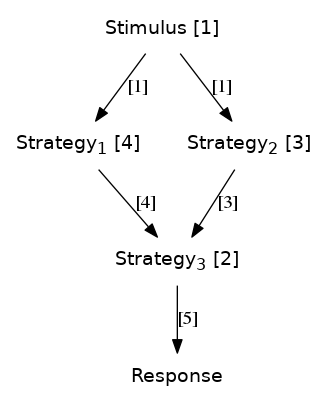
\includegraphics[width=0.4\textwidth]{volr.png}
    \caption{An example learning graph in Volr.}
    \label{volr:graph}
  \end{center}
\end{wrapfigure}

As shown in figure \ref{volr:graph} stimulus, strategies and response are
all associated with an integer that denotes their dimensionality.
The dimensionality is necessary for several reasons:
First, the network needs to learn from a given input, which is
required to adhere to the dimensionality restriction.
Second, the strategies can be combined to provide
networks of different sizes, but the input for those strategies have to
depend on the outputs of the previous layers, which requires them to combine
the features.
The dimensionality of the strategies entirely depends on the number of
elementary functions (\texttt{functions}) associated with the strategy.
Figure \ref{volr:graph} shows an example of this. Here, a singly dimensional
input is fed into two strategies with four and three EFs respectively. They are
then combined into a 7-dimensional input, which is reduced to five in the last
strategy, and forwarded to the response.

Stimuli and response sections further specify a file, from which the input data
and expected output data is read. This is used to train the network according
to the given data.

Responses also allow to specify learning rates (\texttt{learning\_rate}) to
adjust the learning rate of the underlying implementation.

A 3- and 4-layer network can be seen in appendix \ref{volr:example}.

{\let\clearpage\relax\chapter{Case study: Krechevsky maze}}
\label{case}

This case study is based on the mazes built by Krechevsky in the
1930's \autocite{Krechevsky1932}. Krechevsky researched the behaviour of
rats by guiding them through carefully constructed mazes that gave the rats
clues in the form of shapes and colours of light \autocite{Krechevsky1932}. Each
fork showed one or more of the features, leading either to success (reward)
or failure (blocked path). To illustrate such a maze, imagine a bright lamp
being consistently installed at paths leading to reward, while complete
darkness consistently points to dead ends. Here the rats would quickly learn
to follow the lit paths to claim their reward \autocite{Krechevsky1932}.
For the cognitive neurosciences this experiment is interesting, because it is
feasible to introspect each maze decision and compare the decisions of the
virtual system with real rats.

Incidentally the mazes are easy to model because the features can be represented
with simple boolean flags when they are present (\texttt{1}) or absent (\texttt{0}).
Therefore, a simple maze with only T-junctions can be generated by showing the "rat"
an array of input features and expecting it to make a choice: left or right.

\section{Experiment result}
The Krechevsky maze in the experiment is a simple two-feature maze with
a single branching option, to give an immediate feedback for the learning
network. For the sake of the experiment, the features in the maze are entirely
consistent. A perfect network is thus expected to achieve a 100\% accuracy.

Two networks were constructed to calculate the data: a 3-layer and 4-layer
maze. Both use a sample size of 500.

\begin{table}
  \centering
  \begin{tabular}{l c c}
    & \textbf{3 layers} & \textbf{4 layers} \\
    Runtime & 40.505ms & 49.137ms \\
    Accuracy & 100\% & 100\%
  \end{tabular}

  \caption{Runtimes of volr networks in milliseconds, averaged over 100 runs.}
  \label{case:runtimes}
\end{table}

The results are shown in table \ref{case:runtimes}. Both networks achieve
a 100\% accuracy, which indicates that they are capable of learning the task
at hand.
Information about the execution and runtime environment can be found in
appendix \ref{env}.

\chapter{Discussion}
This paper set out to examine whether a DSL can model meaningful machine
learning tasks for the cognitive neurosciences. Building on
relevant theory from cognitive science and computer science, a DSL, Volr,
was presented. A backend executing to OpenCL was implemented and a
Krechevsky-like maze was constructed and evaluated through two 3- and
4-layered neural networks with backpropagation and gradient descent learning.

The evaluation showed that Volr successfully modelled the Krechevsky-maze
task with different network configurations, and with the expected accuracy.

The result is encouraging because it is easily scaleable to more complex
mazes and other problems. The present study only examined a perfect maze where
each feature was consistent. A possible extension of this would be to randomize the
features and study the behaviour of the system. Similarly, this system could
allow to support a form of "memory" where previous decisions are stored as
\textit{breadcrumbs}, that can assist the virtual rat in its decision.

With the concept of memory, the virtual model would be even closer to the biological model
and its learning mechanism. This underlines the present work as an initial
effort towards more elaborate modelling tools.

Reviewing the hypothesis two shortcomings became apparent during the evaluation:
accurately representing the \ref{ref} model in the DSL and modelling
the mechanisms of the biological substrate.

Notably two features from the \ref{ref} model were ignored in the paper: the
GAS and the comparator. The GAS was partly implemented by the supervised
learning strategy, in which the stochastic gradient descent learning
continually improved the network towards the training data.
But the model does not have control over the GAS and the mechanisms with
which the network is improved.
A more fitting approach to capture the GAS could be to implement
reinforcement learning, where the goal is more clearly stated.
The comparator was omitted because it required the
implementation of multiple and competing strategies. This is however
easier to mitigate by simply constructing multiple models and choosing
the best network, based on some criterion.

Another shortcoming of the approach is the Futhark implementation backed
by traditional machine learning perceptron networks. These networks cannot
accurately model neurons in the biological brain. The layered approach does not allow
for the continuous feedback from neighbouring strategies, nor for the
asynchronous workings of the neurons. A mediation of this could be to
write a backend which supports such a clustered neuronal base, similar to
the idea of the EF in the \gls{ref} model. Neuromorphic hardware would be
particularly interesting to examine here, because they are capable of
simulating exactly these properties.

\clearpage

\printglossary

\appendix

\chapter{Volr EBNF}
\label{ebnf}

A railroad diagram of the below EBNF is available online at
\url{https://github.com/Jegp/volr-report/blob/master/railroad.png}.

\begin{verbatim}
  model = ( stimulus | strategy | response )
        , { [ space ] , "," , [ space ] , ( stimulus | strategy | response ) };

  stimulus = "stimulus" , [ space ] , name , [ space ] , dimensionality
           , [ space ] , "file:" , [ space ] , name;
  strategy = "strategy" , [ space ] , name , [ space ] , input
           , [ space ] , "functions:" , [ space ] , integer;
  response = "response" , [ space ] , dimensionality , [ space ] , input
           , [ space ] , "file:" , [ space ] , name
           , [ space ] , "learning_rate:" , [ space ] , number;

  input = "from" , [ space ] , name , { [ space ] , name };
  dimensionality = "[" , [ space ] , integer , [ space ] , "]";

  name list = name , { [ space ] , "," , name };
  name = letter , { letter | digit };
  letter = ? non-whitespace Unicode character ?;
  space = space character , { space character };
  space character = ? white space character ?;

  number = integer , ["." , digit , {digit}];
  integer = ["-"] , digit , {digit};
  digit = "0" | "1" | "2" | "3" | "4"
        | "5" | "6" | "7" | "8" | "9";
\end{verbatim}

\clearpage

\chapter{3- and 4-layer learning networks in Volr}
\label{volr:example}

\lstinputlisting{two_features.volr}

\chapter{Benchmark informations}
\label{env}
The benchmark was executed on an Asus X550VX with an Intel i7 6700HQ 2.6GHz
quad-core processor, 8 GB of DDR4 2133 MHz SDRAM and an NVIDIA GeForce GTX 950M
(640 CUDA cores at 914MHz).

The benchmark was run by the following command (standing in the directory of
the volr project):
\begin{verbatim}
volr -f examples/4layer_500.volr
\end{verbatim}

Runtimes was extracted using a specific \texttt{-t} flag in the Futhark
runtime, and re-run 100 times with the Futhark \texttt{-r} flag. The above
command produces binaries in the \texttt{bin} folder, allowing us to execute
100 iterations and put the results into the \texttt{times.txt} file:
\begin{verbatim}
cat examples/maze_x500.txt examples/maze_y500.txt \
  | bin/futhark-model -r 100 -t times.txt
\end{verbatim}

\printbibliography

\end{document}
